\chapter{Introduction}
\label{introduction}


%\section{Introduction}

%{\color{red} \textbf{  Instruction:} “Introduce the topic of the research and set the foundation for the rest of the work. Begin with a general overview of the subject area, and explain what is being studied and why it matters. Highlight the importance of the chosen field, showing its relevance in academic, industrial, or social contexts.”}

 %\textbf{\color{blue} Example:} Heart disease is one of the \textbf{leading causes of death worldwide}, responsible for \textbf{millions of fatalities} each year. \textbf{Early detection} and \textbf{diagnosis} can significantly reduce \textbf{mortality} by enabling \textbf{timely treatment}. Traditional methods depend heavily on \textbf{manual diagnosis by doctors}, which can be \textbf{time-consuming} and prone to \textbf{human error}. In recent years, \textbf{machine learning (ML)} has emerged as a \textbf{powerful tool} for developing \textbf{automated} and \textbf{accurate prediction systems }[1]. This thesis focuses on building an \textbf{ML-based model} to predict the \textbf{likelihood of heart disease} using \textbf{medical data} such as \textbf{age, blood pressure, cholesterol level}, and other \textbf{clinical factors}. 



\section{Background of the Study} 

{\color{red} \textbf{  Instruction:}  “Give a brief description of how the topic or technology started and how it has evolved over time. Highlight key milestones that shaped its development. Mention important inventions that played a significant role. Discuss major breakthroughs that contributed to its growth and current relevance.”}

 \textbf{\color{blue} Example:} Heart disease research and diagnostic methods \textbf{started} many decades ago and have \textbf{evolved over time} through continuous scientific advancements. Several \textbf{key milestones} shaped its development, including the introduction of \textbf{electrocardiograms (ECG)} and \textbf{cholesterol testing}[2]. Important \textbf{inventions} such as \textbf{advanced imaging techniques} and \textbf{biomarker detection methods} played a significant role in improving diagnosis. Major \textbf{breakthroughs}, including the use of \textbf{machine learning (ML)} for \textbf{predictive modeling}, have contributed to the field’s \textbf{growth} and its \textbf{current relevance} in healthcare[3][4].



\subsection{State of the Art in the Modern Context} 

{\color{red} \textbf{  Instruction:} “Describe the \textbf{current status of the field}, focusing on how it is being used and developed today. Highlight \textbf{recent research contributions, emerging tools}, and \textbf{advanced technologies} that are shaping progress in this area. Discuss the \textbf{current challenges}, such as \textbf{technical limitations, ethical concerns}, or \textbf{practical implementation issues}. Cite a few \textbf{up-to-date research papers or articles} to provide insights into the latest \textbf{developments} and \textbf{trends}.”}

 \textbf{\color{blue} Example:} Today, \textbf{machine learning (ML) models} trained on \textbf{large datasets} can predict \textbf{heart disease risk} with impressive \textbf{accuracy}. Research shows that \textbf{algorithms} such as Random Forest, Support Vector Machines (SVM), and \textbf{deep neural networks} outperform traditional \textbf{scoring systems} like the \textbf{Framingham Risk Score}[5]. Recent studies also incorporate \textbf{hybrid techniques}, such as combining \textbf{feature selection} with \textbf{ensemble learning} to improve \textbf{prediction performance}. Additionally, \textbf{deep learning models} using \textbf{patient ECG signals} and \textbf{wearable sensor data} are being explored in \textbf{current research}, demonstrating ongoing \textbf{innovation} in the field[6].



\subsection{Importance and Relevance of the Topic}

{\color{red} \textbf{  Instruction:} 
“Explain the \textbf{importance of this topic} by emphasizing its \textbf{relevance} and \textbf{impact}. Highlight its \textbf{usefulness} in society, \textbf{industry}, or \textbf{research}, showing how it contributes to \textbf{progress} and \textbf{innovation}. Discuss the \textbf{benefits} that could be achieved by solving this problem, particularly how \textbf{individuals}, \textbf{communities}, or \textbf{organizations} may gain from its solutions.”}


 \textbf{\color{blue} Example:} A heart disease prediction system based on machine learning could be integrated into various healthcare settings to maximize its impact[9]. For example, in rural clinics, it can assist non-specialist doctors by providing quick and reliable risk assessment for both compensating for the shortage of trained cardiologists. In addition, the system can be embedded into mobile health applications through multiple systems, such as healthcare providers, and cardiovascular health conveniently from home. Within hospital usage patterns, such a tool can help prioritize high-cash patients, ensuring that those in urgent need of care receive immediate attention. Beyond these use cases, the system can also reduce the overall diagnostic workload for healthcare professionals, streamline decision-making, and ultimately improve patient outcomes by enabling timely interventions.




%\section{Problem Statement} 
\section{Research Problem and Its Context} 

{\color{red} \textbf{  Instruction:} “Clearly explain the main problem that your work is attempting to solve. Mention any gaps in current systems or existing limitations, and highlight the areas where improvements or solutions are needed.”}

 \textbf{\color{blue} Example:}
 While ML-based heart disease prediction models have shown promising results, many suffer from issues such as overfitting, poor generalization to new data, or reliance on large datasets that are not always available.

This thesis aims to design a model that maintains high prediction accuracy even with small to moderately sized datasets and simple features, while being computationally efficient enough to deploy in low-resource settings [8].


\section{Motivation}

{\color{red} \textbf{  Instruction:} Why this problem is important and worth investigating. Explain the reason the topic was chosen. Mention any personal interest or factors that caused this problem to attract attention.}

 \textbf{\color{blue} Example:} The motivation for pursuing a thesis on heart disease prediction includes:

\begin{itemize}
    \item \textbf{Healthcare Impact:} Contributing to early detection of heart disease to reduce mortality and improve patient outcomes.
    \item \textbf{Technological Advancement:} Applying machine learning techniques to solve real-world healthcare problems.
    \item \textbf{Resource Optimization:} Creating a system that is efficient and usable even in low-resource or rural settings.
    \item \textbf{Research Contribution:} Advancing knowledge in medical AI and providing a foundation for future studies.
    \item \textbf{Practical Application:} Preparing a deployable system that can assist healthcare professionals and patients in decision-making.
    \item \textbf{Data-Driven Insight:} Leveraging clinical and demographic data to develop predictive models for accurate diagnosis.
\end{itemize}

\section{Applications and Practical Use Cases}

{\color{red} \textbf{  Instruction:} Real-world or academic use cases of your research. "Describe the potential real-life applications of the research. Highlight its use in areas such as industry, healthcare, education, or other relevant fields."}

 \textbf{\color{blue} Example:} A heart disease prediction system based on machine learning could be integrated into various healthcare settings to maximize its impact[9]. For example, in rural clinics, it can assist non-specialist doctors by providing quick and reliable risk assessment for both compensating for the shortage of trained cardiologists. In addition, the system can be embedded into mobile health applications through multiple systems, such as healthcare providers, and cardiovascular health conveniently from home. Within hospital usage patterns, such a tool can help prioritize high-cash patients, ensuring that those in urgent need of care receive immediate attention. Beyond these use cases, the system can also reduce the overall diagnostic workload for healthcare professionals, streamline decision-making, and ultimately improve patient outcomes by enabling timely interventions.

\section{Research Objectives }
{\color{red} \textbf{  Instruction:} Clearly define the primary aim and sub-goals of your study. "To interpret the aims of the research. Write one general objective and two to three specific objectives to outline the intended outcomes and focus areas of the study."}

 \textbf{\color{blue} Example:} 
 
 \textbf{General Objective:}
To develop an accurate and reliable machine learning model for predicting heart disease.

\textbf{Specific Objectives:}
To collect and preprocess clinical and demographic data relevant to heart disease.

To identify and select the most important features that influence heart disease prediction.

To design, train, and evaluate different machine learning models to determine the most effective approach.

\section{Research Methodology (Overview) }
{\color{red} \textbf{  Instruction:} "A brief overview of the research methods or approaches used." You can add a conceptual diagram.}

 \textbf{\color{blue} Example:} A simple attack Classification is presented in Fig: \ref{fig:mlpipeline}.

\begin{figure}[ht]
    \centering
    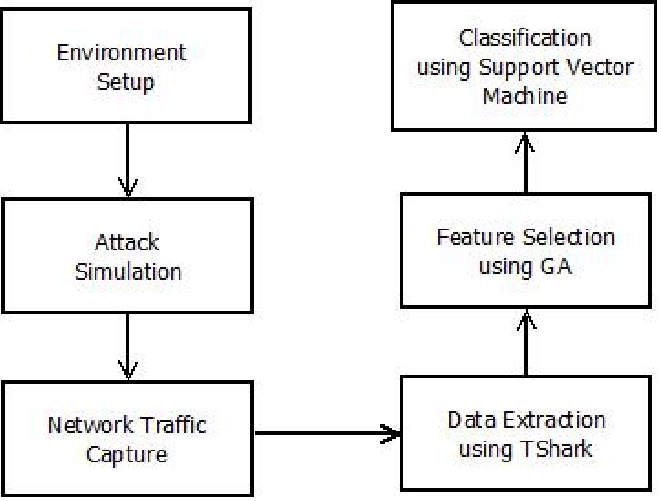
\includegraphics[width=0.80\textwidth]{Images/Block-diagram.png}
    \caption{Block Diagram of the Classification System}
    \label{fig:mlpipeline}
\end{figure}


 

%
%\begin{equation}
%\text{Accuracy} = \frac{TP + TN}{TP + TN + FP + FN}
%\tag{1.1}
%\end{equation}


%\begin{table}[H]
%\centering
%\caption{Sample UCI Heart Disease dataset}
%\begin{tabular}{|c|c|p{1.5cm}|c|p{1.5cm}|c|c|c|p{1.5cm}|}
%\hline
%\textbf{Age} & \textbf{Sex} & \textbf{Chest Pain Type} & \textbf{RestBP} & \textbf{Chole sterol} & \textbf{FastingBS} & \textbf{RestECG} & \textbf{MaxHR} & \textbf{Heart Disease} \\ \hline
%63 & 1 & 3 & 145 & 233 & 1 & 0 & 150 & 1 \\ \hline
%37 & 1 & 2 & 130 & 250 & 0 & 1 & 187 & 0 \\ \hline
%41 & 0 & 1 & 130 & 204 & 0 & 0 & 172 & 0 \\ \hline
%\end{tabular}
%\end{table}


\section{Research Contribution}

{\color{red} \textbf{  Instruction:} “Highlight what is new or unique in the work by mentioning any improvements, comparisons, or simplifications introduced.”}

 \textbf{\color{blue} Example:} Several key contributions were made by this research. A comparison of multiple machine learning algorithms was provided on the same dataset using a minimal set of features, and their relative performance was highlighted.


\section{Financial Planning and Timeline}

\subsection{ Budget Estimation}

{\color{red} \textbf{  Instruction:} Break down the costs of your work if it involves hardware, software, or travel. If costs are not applicable, skip this part or write: “No major cost is involved.”}

 \textbf{\color{blue} Example:} No major costs are involved in this work. All tools and datasets used are open-source and freely available. The development environment runs on a personal laptop.

\subsection{  Gantt Chart }
{\color{red} \textbf{  Instruction:} "Create a visual chart showing your research timeline (tasks vs. weeks/months)".}

 \textbf{\color{blue} Example:} The Fig \ref{fig:planschedule} represents a visual chart of the research timeline for a heart disease prediction project. It outlines the sequence of key tasks, including data collection, data pre-processing, feature selection, model development, training and validation, performance analysis, and deployment preparation. Each task is mapped along a timeline to show the planned duration and order of activities, helping to organize the workflow and track progress throughout the study.


\begin{figure}[ht]
    \centering
    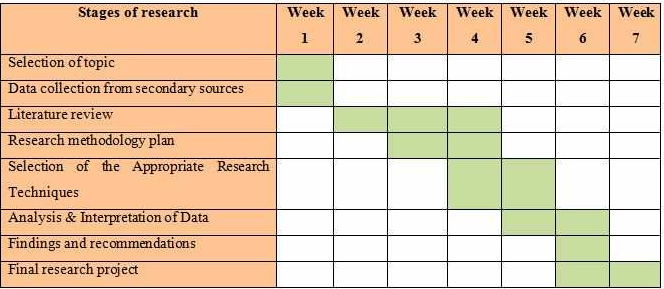
\includegraphics[width=0.90\textwidth]{Images/A planned thesis schedule.png}
    \caption{A planned thesis schedule.}
    \label{fig:planschedule}
\end{figure}



\section{Organization of the Dissertation }

\textbf{\color{blue} Example:}

In this dissertation, the remaining chapters are organized as follows:

Chapter \ref{Literature Review}, \textit{Literature Review}, discusses the existing research related to heart disease prediction. It provides an overview of various machine learning techniques and compares their relative effectiveness in predicting heart diseases.

Chapter \ref{System Architecture}, \textit{Methodology}, describes the dataset employed in this study, the applied feature selection techniques, the process of model development, and the evaluation strategies adopted to assess performance.

Chapter \ref{Results and Discussion}, \textit{Results and Discussion}, presents the experimental outcomes along with graphical representations and offers a comprehensive analysis of the model's predictive performance.

Finally, Chapter \ref{Conclusion}, \textit{Conclusion and Future Work}, summarizes the key findings of this research, outlines its limitations, and provides recommendations for future work and potential improvements.
